\addcontentsline{toc}{section}{Appendix}
% \usepackage{multirow}
% \usepackage{graphicx}

\chead{\textit{\nouppercase{Appendix}}}

\thispagestyle{plain} % surpress header on first page

\subsection{Appendix A: Tables}
\thispagestyle{plain} % surpress header on first page




\phantom{This text will be invisible}
\hspace{20cm}
% Please add the following required packages to your document preamble:
% \usepackage{multirow}
% \usepackage{graphicx}
\begin{table}[H]
\centering
\caption{Parameterization of \cite{keane1994SolutionEstimationDiscrete} model}\label{tab:1}
\resizebox{\textwidth}{!}{%
\begin{tabular}{lcccl}
\hline
Category                     & Parameter     & Value   & Standard Error & Definition                                   \\ \hline
General                      & $\delta$      & 0.95    & 0.000616       & discount factor                              \\ \hline
\multirow{6}{*}{Blue-collar} & $\alpha_{10}$ & 9.21    & 0.011858       & log of rental price                          \\
                             & $\alpha_{11}$ & 0.038   & 0.001045       & return to an additional year of schooling    \\
                             & $\alpha_{12}$ & 0.033   & 0.000444       & return to same sector experience             \\
                             & $\alpha_{13}$ & -0.0005 & 0.000012       & return to same sector, quadratic experience  \\
                             & $\alpha_{14}$ & 0.0     & 0.000738       & return to other sector experience            \\
                             & $\alpha_{15}$ & 0.0     & 0.000029       & return to other sector, quadratic experience \\ \hline
\multirow{6}{*}{White collar} & $\alpha_{20}$ & 8.48 & 0.005998   & log of rental price                    \\
                             & $\alpha_{21}$ & 0.07    & 0.000344       & return to an additional year of schooling    \\
                             & $\alpha_{22}$ & 0.067   & 0.000546       & return to same sector experience             \\
                             & $\alpha_{23}$ & -0.001  & 0.000016       & return to same sector, quadratic experience  \\
                             & $\alpha_{24}$ & 0.022   & 0.00033        & return to other sector experience            \\
                             & $\alpha_{25}$ & -0.0005 & 0.000022       & return to other sector, quadratic experience \\ \hline
\multirow{3}{*}{Education}    & $\beta_0$     & 0.0  & 244.837595 & constant reward for choosing education \\
                             & $\beta_1$     & 0.0     & 134.591673     & reward for going to college (tuition, etc.)  \\
                             & $\beta_2$     & -4000   & 209.14159      & reward for going back to school              \\ \hline
Home                         & $\gamma_0$     & 17750   & 270.436557     & constant reward of non-market alternative    \\ \hline
\end{tabular}%
}
\end{table}









\newpage
\subsection{Appendix B: Figures}
\thispagestyle{plain} % surpress header on first page




\vspace{10mm} %5mm vertical space
\begin{figure}[H]
	\caption{Decision tree \label{fig:1}}
	\centering
	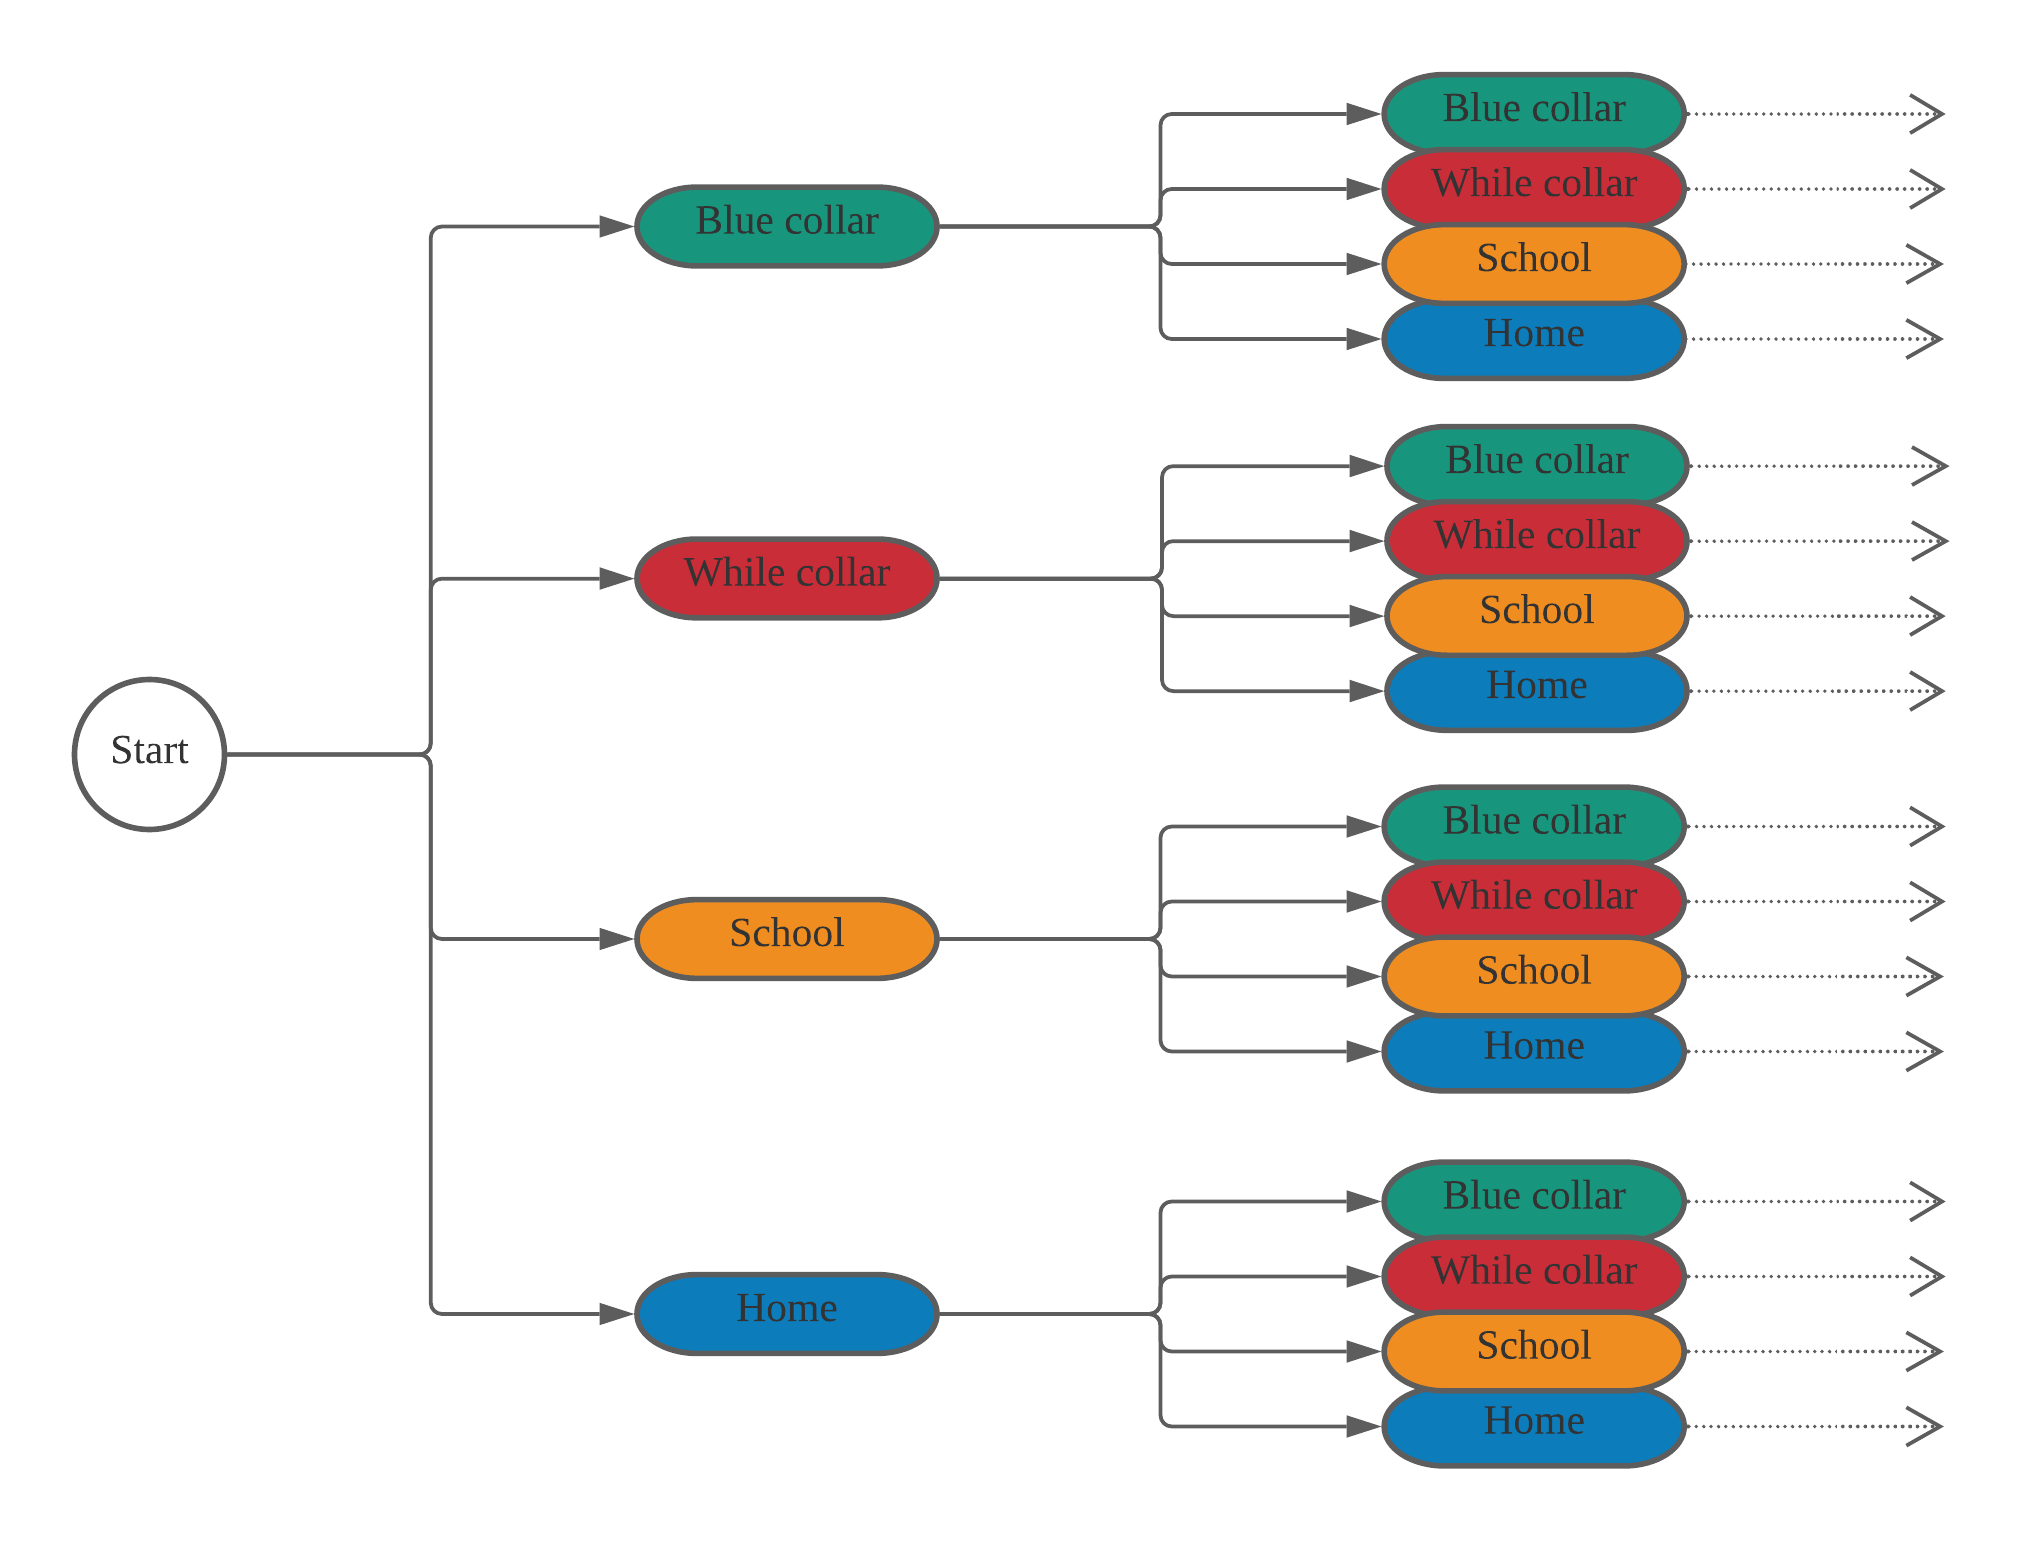
\includegraphics[scale=1]{./resources/kw94-decisiontree}
	\label{fig:corr}
\end{figure}

\vspace{10mm} %5mm vertical space
\begin{figure}[H]
	\caption{Heat map of selective parameters \label{fig:2}}
	\centering
	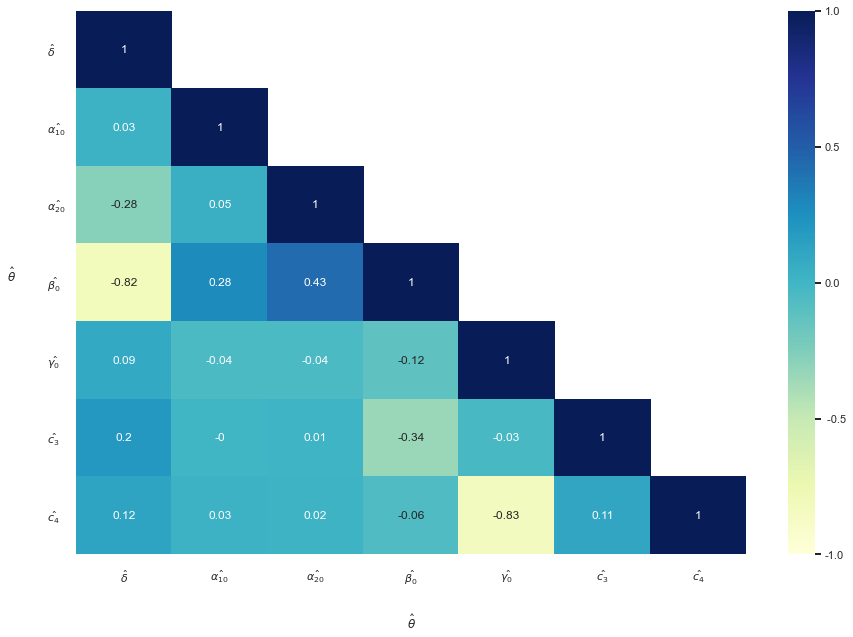
\includegraphics[scale=0.5]{./resources/heatmap}
	\label{fig:corr}
\end{figure}


\vspace{10mm} %5mm vertical space
\begin{figure}[H]
	\caption{ Comparison of shares of occupation decisions over time between scenarios\label{fig:3}}
	\centering
	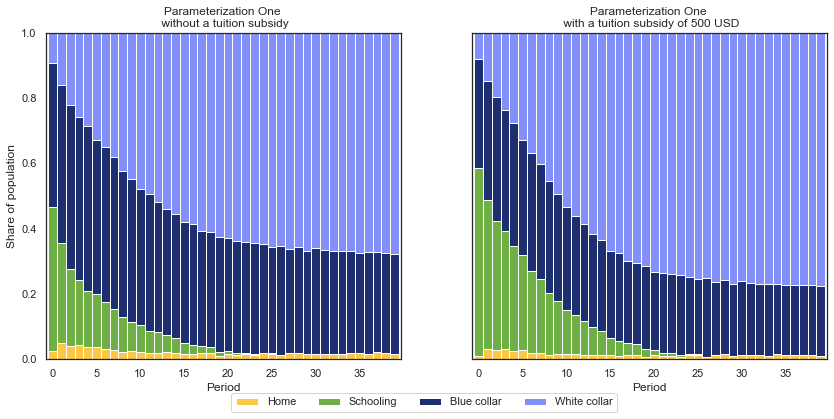
\includegraphics[scale=0.5]{./resources/choiceovertime}
	\label{fig:corr}
\end{figure}

\vspace{10mm} %5mm vertical space
\begin{figure}[H]
	\caption{Probability distribution of QoI\label{fig:4}}
	\centering
	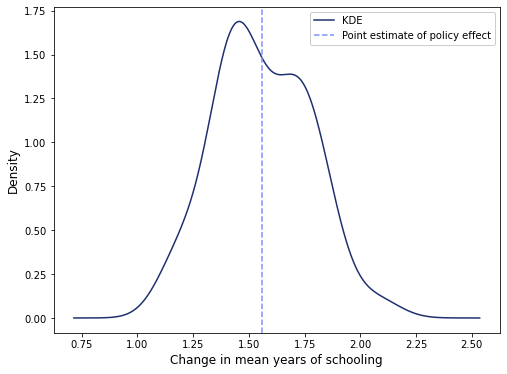
\includegraphics[scale=0.5]{./resources/qoi}
	\label{fig:corr}
\end{figure}


\vspace{10mm} %5mm vertical space
\begin{figure}[H]
	\caption{PDF of output for SA \label{fig:5}}
	\centering
	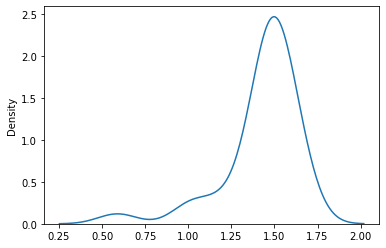
\includegraphics[scale=0.7]{./resources/qoi-SA}
	\label{fig:corr}
\end{figure}


\vspace{10mm} %5mm vertical space
\begin{figure}[H]
	\caption{ Quantile-base sensitivity measures on \cite{keane1994SolutionEstimationDiscrete} model\label{fig:6}}
	\centering
	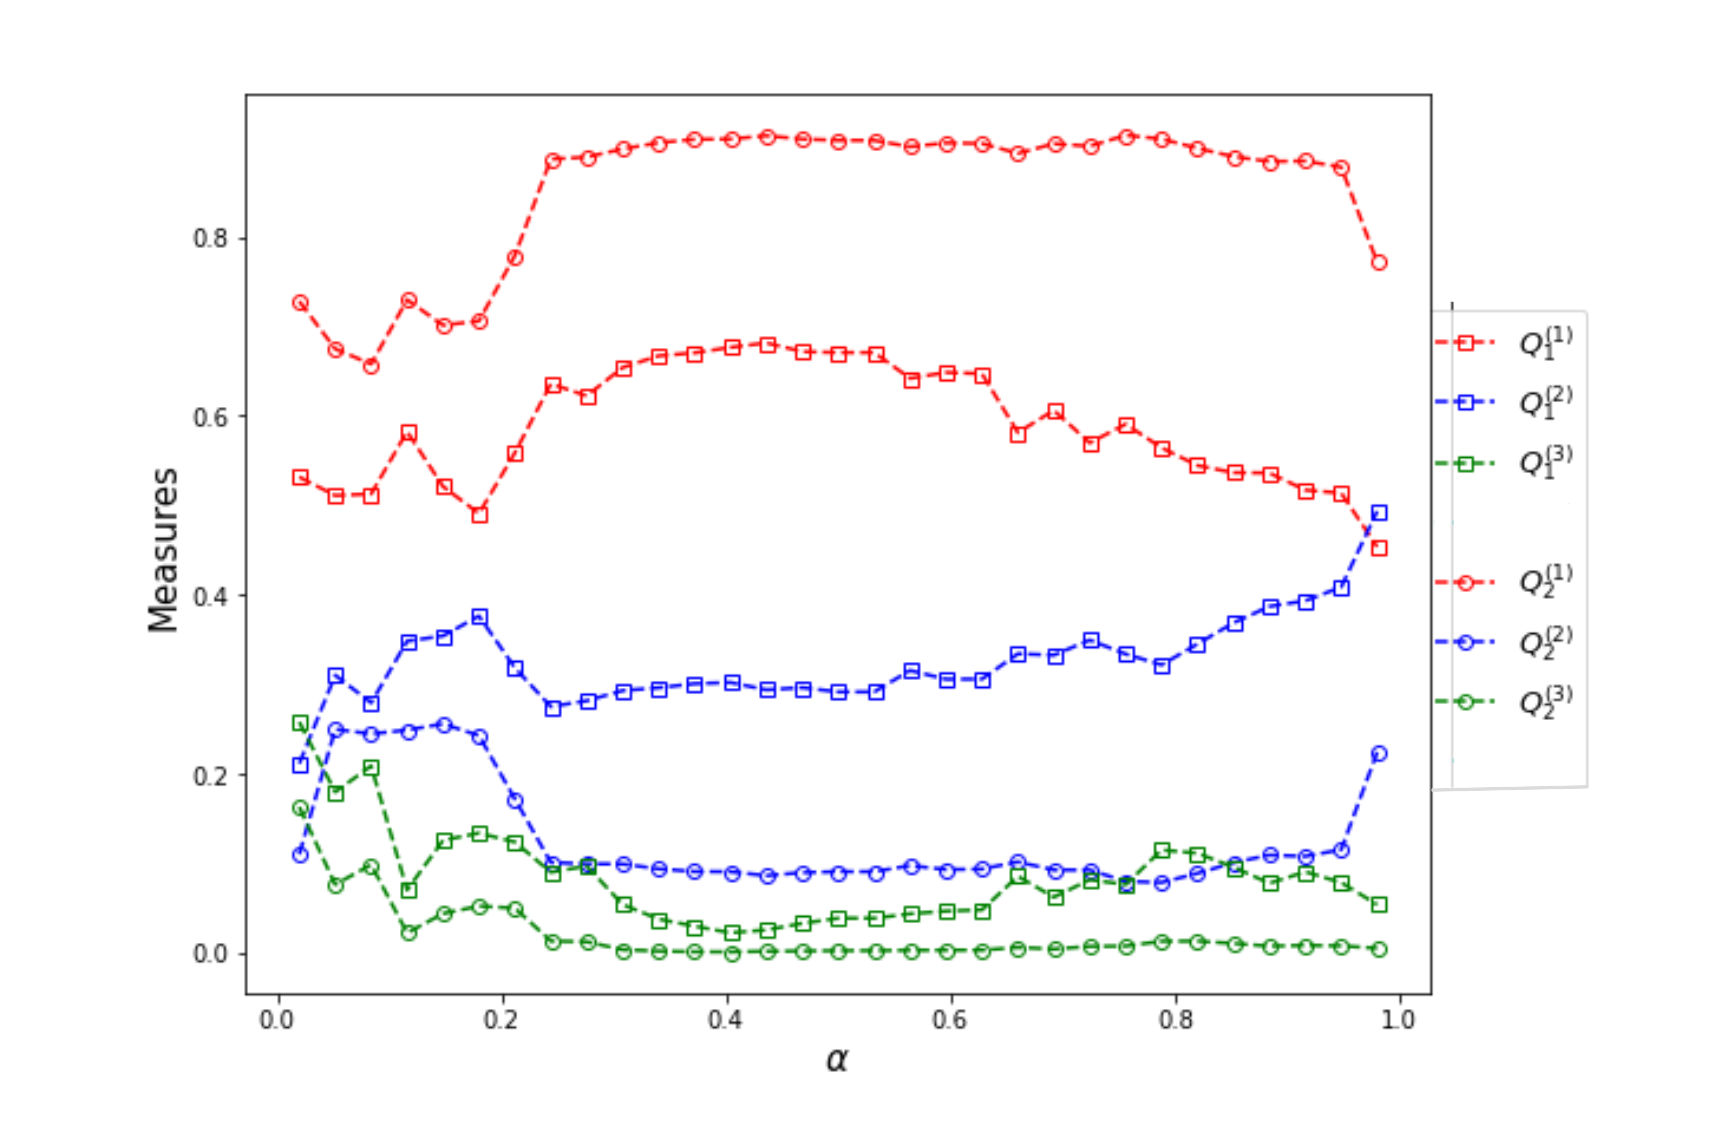
\includegraphics[scale=0.3]{./resources/QBSM}
	\label{fig:corr}
\end{figure}